\documentclass[10pt,a4paper]{article}
\usepackage[utf8]{inputenc}
\usepackage{amsmath}
\usepackage{amsfonts}
\usepackage{amssymb}
\usepackage{geometry}
\usepackage{calc}
\usepackage{subcaption}
\usepackage{graphicx}
\usepackage{hyperref}
\usepackage{listings}

\usepackage{color}

\definecolor{pblue}{rgb}{0.13,0.13,1}
\definecolor{pgreen}{rgb}{0,0.5,0}
\definecolor{pred}{rgb}{0.9,0,0}
\definecolor{pgrey}{rgb}{0.46,0.45,0.48}
\usepackage{xcolor}

\definecolor{codegreen}{rgb}{0,0.6,0}
\definecolor{codegray}{rgb}{0.5,0.5,0.5}
\definecolor{codepurple}{rgb}{0.58,0,0.82}
\definecolor{backcolour}{rgb}{0.95,0.95,0.92}

\lstdefinestyle{mystyle}{  
    commentstyle=\color{codegreen},
    keywordstyle=\color{magenta},
    numberstyle=\tiny\color{codegray},
    stringstyle=\color{codepurple},
    basicstyle=\ttfamily\footnotesize,
    breakatwhitespace=false,         
    breaklines=true,                 
    captionpos=b,                    
    keepspaces=true,                 
    numbers=left,                    
    numbersep=5pt,                  
    showspaces=false,                
    showstringspaces=false,
    showtabs=false,                  
    tabsize=2
}


\lstset{style=mystyle}
 

\def\LRA{\Leftrightarrow\mkern40mu}

%\geometry{hmargin=1.5cm,vmargin=1.5cm}

\author{Cartron Mathurin}
\title{Compte Rendu du projet d'informatique 3-1}


\begin{document}

\maketitle
\tableofcontents

\section{Le choix du jeu}
Pour ce qui est du choix du jeu j'ai penser comme si ce n'était pas un projet de cours. Je me suis demandé ce à quoi j'aimerais le plus jouer et celui que je pourrais le plus modifier pour y ajouter "ma patte". Je suis donc partie sur le model de \textit{Excit} en me disant que j'en ferai un jeu avec de la narration. Chaque niveau étant un chapitre d'une histoire. Histoire qui à inspiré le nom du jeu \textit{Cheat sheet}, qui se traduirait par \textit{Anti-sèche}. L'idée était d'aider Mathurin à aller à son partiel, il était dans son appartement et devait sortir avant d'être en retard, ce qui explique que le score diminue au fur et à mesure que le temps s'écoule. Chaque niveau représentait une matière de ce semestre, et il était possible de récupérer des items, comme des antisèches, qui donnaient un bonus de score, ou des livre de cours qui eux donnaient des malus. Finalement la programmation de malus et de bonus n'étant pas au point j'ai préféré me concentrer sur l'éditeur plutôt que de tout faire au détriment des autre matières.
\begin{figure}[h!]
\begin{subfigure}{.24\textwidth}
	\centering
	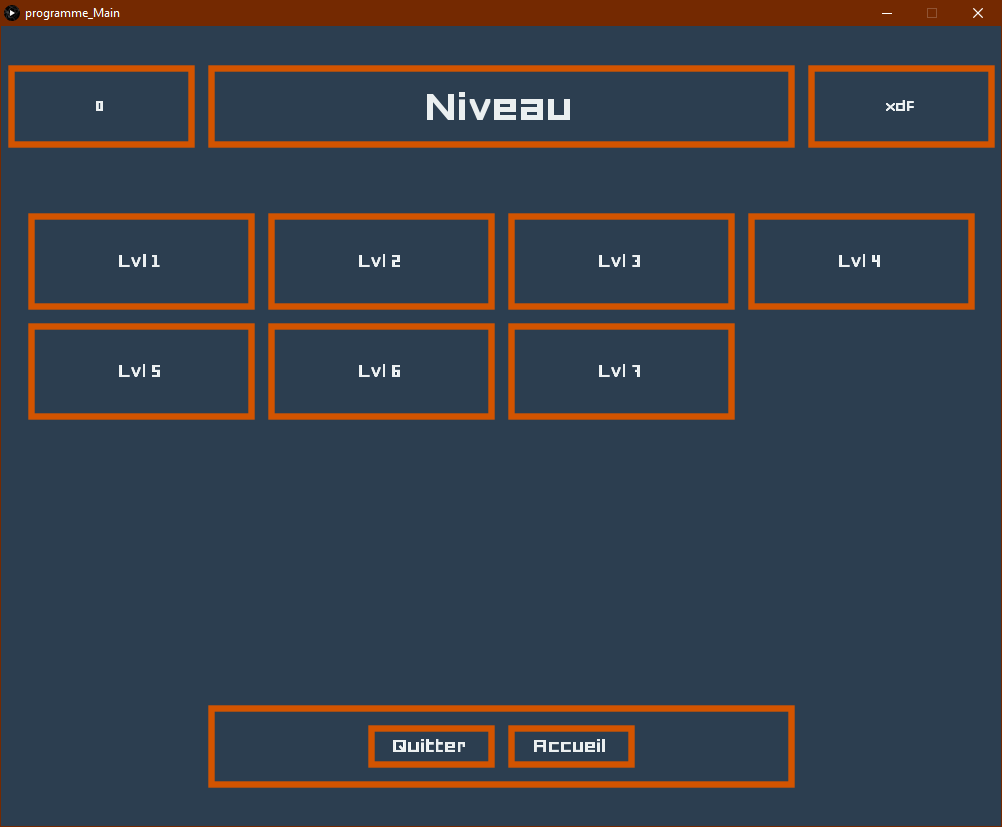
\includegraphics[width=.9\linewidth]{Capture1.PNG}
\end{subfigure}
\begin{subfigure}{.24\textwidth}
	\centering
	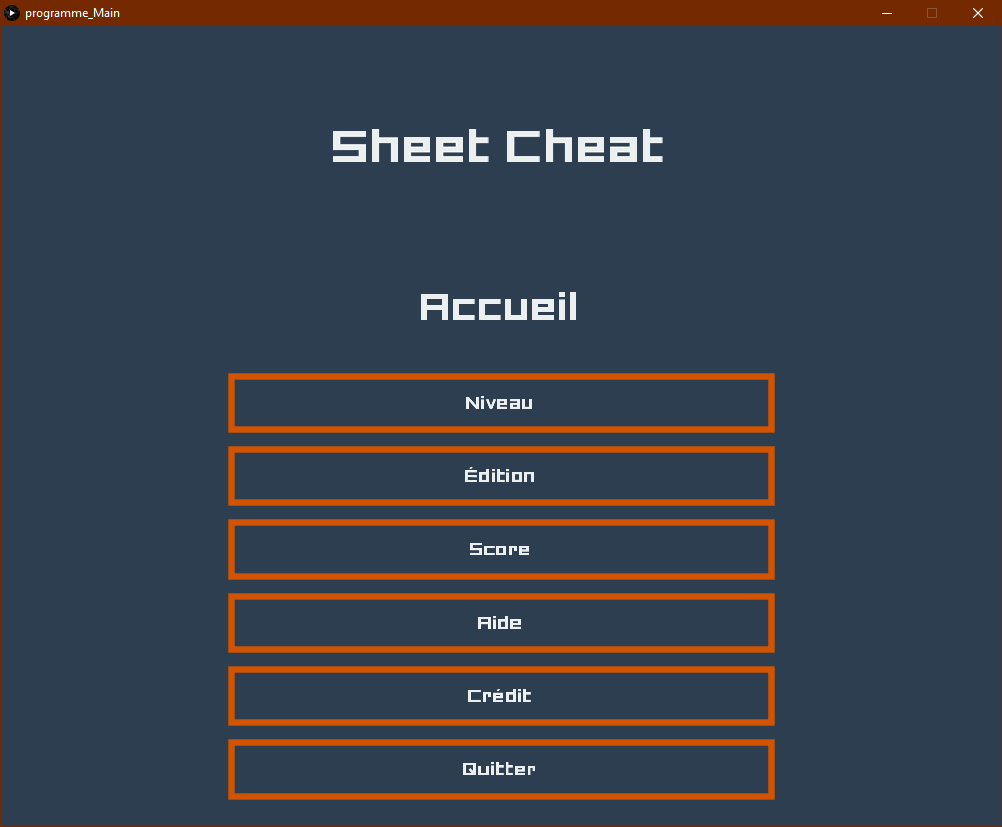
\includegraphics[width=.9\linewidth]{Capture2.PNG}
\end{subfigure}
\begin{subfigure}{.24\textwidth}
	\centering
	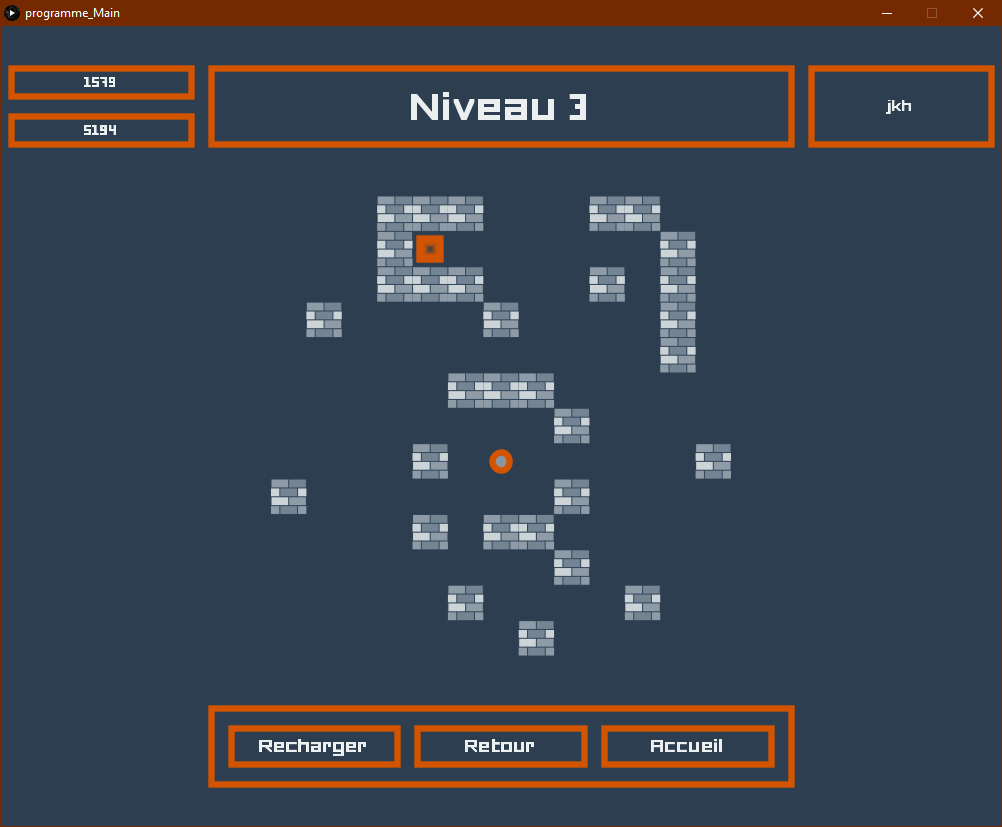
\includegraphics[width=.9\linewidth]{Capture3.PNG}
\end{subfigure} 
\begin{subfigure}{.24\textwidth}
	\centering
	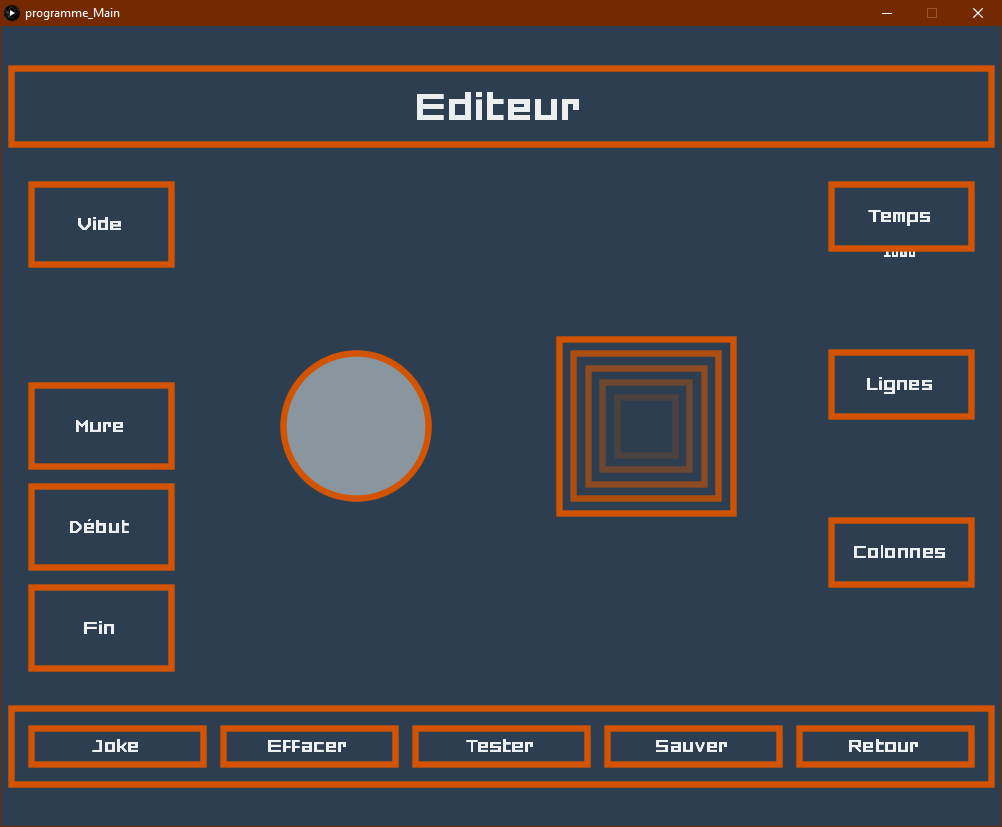
\includegraphics[width=.9\linewidth]{Capture4.PNG}
\end{subfigure}
\label{fig10}
\caption{Image du jeu}
\end{figure}
\paragraph{Attention}Les capture d'écrans ont été effectué pendant la réalisation du code, par nostalgie je les aient laissées. 
\section{La programmation}
Au vue de la taille du projet, il était impératif de découpé le projet. Je sais que certain on commencé par le \textit{jeu} en tant que telle, pour ma part j'avais peur de coder le jeu et de me retrouver bloqué au moment il aurait fallut l'implémenter dans des pages, avec des menu, etc. J'ai donc commencé par faire les pages et les \textit{boites} qui sont inspiré de mon expérience avec le HTML. 
\subsection{Les commentaires} Comme il est difficile de bien expliquer un programme surtout en 5 pages sans le survoler et sans trop rentrer dans les détailles, je me suis appliqué à commenter le plus clairement possible mon code, je ne vais donc pas faire un doublon avec les commentaires et parler ici de la manière dont j'ai penser mon programme et des choix que j'ai fais. 
\subsection{L'habitude} Le plus gros problème que j'ai eu est que je n'avais jamais travaillé sur un projet de cette ampleur, ainsi ma manière de programmer ressemblait beaucoup à ceci : je programme depuis ce que j'ai mis sur un petit bout de papier en gribouillages, je m'applique, je teste et la, ça ne fonctionne pas. Je débug, je modifie par ci par la, jusqu'à ce que cela marche pour que une fois que ça marche je ne sais même pas pourquoi. Donc mètre le code au propre c'est révélé complexe. Raison pour laquelle il se peux qu'il y ai encore du code inutile. Malgré les nombreuse relecture.
\subsection{La manière de travailler}
Je n'avais pas de réelle méthodologie pour faire en sorte que mon code soit "évolutif". Le moindre ajout d'un fonctionnalité fût un enfer à faire. Sauf si je l'avais prévus à l'avance. De cette manière pour la fin de mon travail je me suis mis à imaginé tout les idées les plus farfelus des le début pour ne pas me retrouvé bloqué. Sauf que cela créer autant de problèmes, notamment une grosse quantité de code inutile.
\subsection{Les éléments du programme }
\subsubsection{Les pages et les boites}
J'ai vu mon programme comme un site HTML, cf Figure \ref{fig1}, contenant un ensemble de pages, contenant elle même un ensemble de boites. Les boites avaient des dimensions et des position unique qu'elles transmettais à ce qu'elle contenaient. Imaginons que je fasse un menu que je mette dans la première page, et que je me rende compte qu'il est trop petit, je n'ai qu'à changer les dimensions de la boite qui contient le dit menu. 
\begin{figure}[h!]
	\centering
	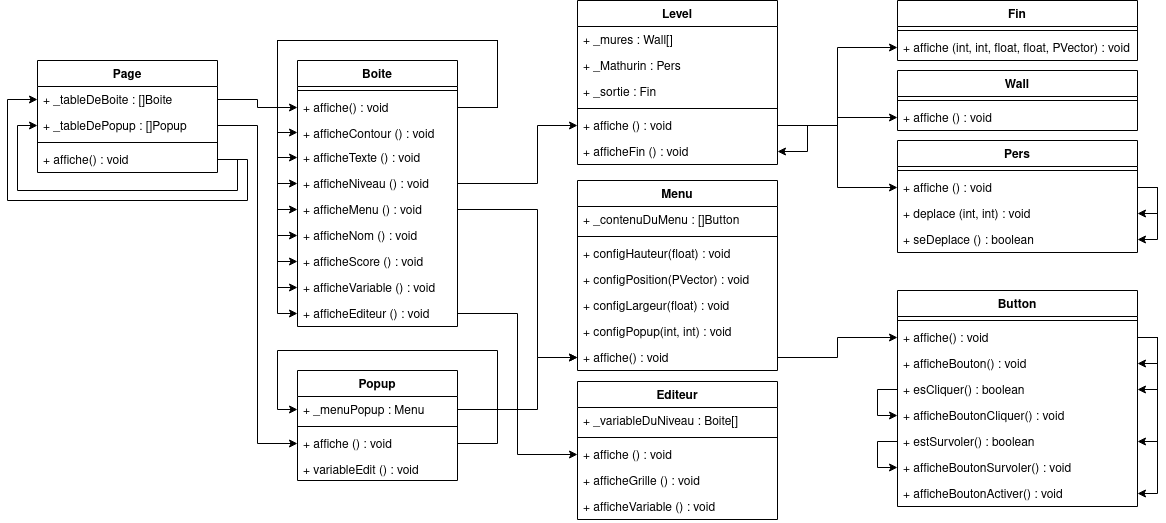
\includegraphics[width=0.9\textwidth]{Affichage .png}
  	\caption{Diagramme uml de l'affichage du jeu}
  	\label{fig4}
\end{figure}
J'ai fais un diagramme UML qui ne contient que la partie affichage de mon programme, cf Figure \ref{fig4}. Mais ce que l'on constate c'est que c'est un fois quand le code de \textit{Boite} que l'on à un \textit{aiguillage} de ce que l'on affiche en fonction de ce que contient la boite. J'ai cependant remarque de ma façon de faire a changé au cours de la programmation. En effet je me disait que c'est lors que l'appelle de la méthode d'affichage d'un objet que je devais transmettre les dimensions, j'avais donc fais des setters que j'appelais à chaque affichage, ce qui consomme beaucoup de ressources. Je suis passé à une autre approche qui consistait à réglé les valeurs des dimensions de la boite "parent" lors de la création de l'objet. Seul inconvénient c'est que la boite n'est pas "redimentionnable". 
\begin{figure}[h!]
\begin{subfigure}{.4\textwidth}
	\centering
	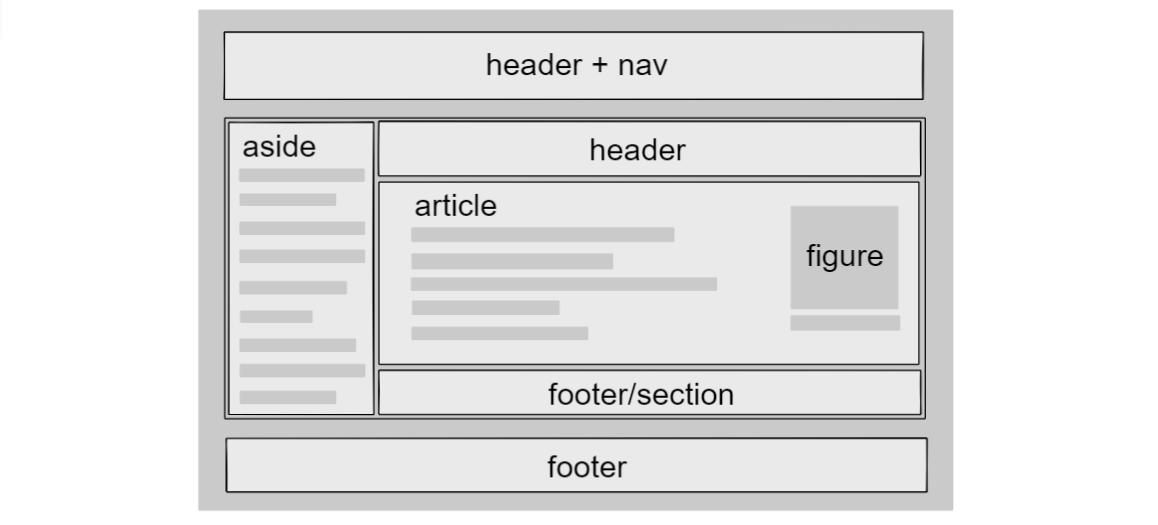
\includegraphics[width=.9\linewidth]{html.png}
  	\caption{gestion de la mise en page des pages html}
  	\label{fig1}
\end{subfigure}
\begin{subfigure}{.25\textwidth}
	\centering
	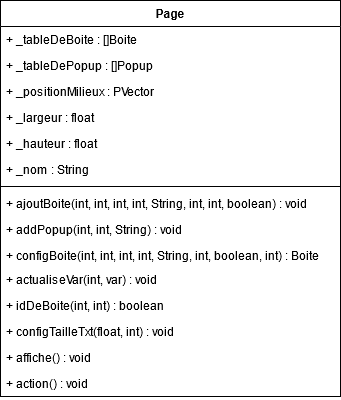
\includegraphics[width=.9\linewidth]{Page.png}
  	\caption{Représentation UML de la class PAGE}
  	\label{fi2}
\end{subfigure}
\begin{subfigure}{.25\textwidth}
	\centering
	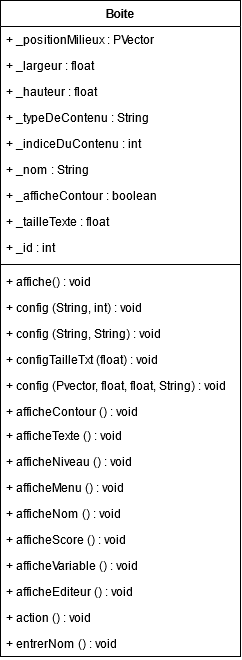
\includegraphics[width=.9\linewidth]{Boite.png}
  	\caption{Représentation UML de la class BOITE}
  	\label{fig3}
\end{subfigure}
\caption{Schémas de compréhension du système de page et de boite}
\label{fig7}
\end{figure}
\subsubsection{les menus et les boutons}
Les menus et les boutons sont des classes que j'ai pensé pour une utilisation plus complexe que je ne le fais ici. En effet de la même manière que une page contient des boites, ici un menu contient des boutons. Il suffit de lier un menu à une boite pour que celle ci la contienne et l'affiche. Lorsque l'on instancie un menu il lui faut un nom le nombre de ligne et de colonne de bouton qu'il va contenir. Puis pour l'ajout d'un bouton, la méthode \textit{ajoutBouton} instancie un bouton de sorte qu'il soit de la bonne dimensions et que la position de celui ci en pixel par rapport au référentiel de processing soit bon. Il ne lui faut que le nom du bouton le type de bouton (Page, Popup, etc) et la position dans le menu. De plus un même menu peut être implémenter dans plusieurs boite en s'actualisant sur les dimensions de la boite qui le contient.
\subsubsection{Le jeu}
Le jeu est en fait une table de niveau générés depuis un fichier texte. Chaque niveau est vu comme un ensemble d'objet, comme les murs le début et la fin. Le personnage se déplace, librement et retourne au début quand il sort de l'espace de jeu. J'ai voulu que les différent objet parlent entre eux mais j'ai eu beaucoup de mal à le faire. J'ai donc centraliser toutes les "discussions" dans la class Level. J'ai penser faire une fonction qui prendrais en compte toutes les dimensions de déplacement possible (gauche, droite, haut, bas) mais comme il n'y à que 4 cas j'ai préféré faire un \textit{switch/case} plus simple. 
\begin{figure}[h!]
	\centering
	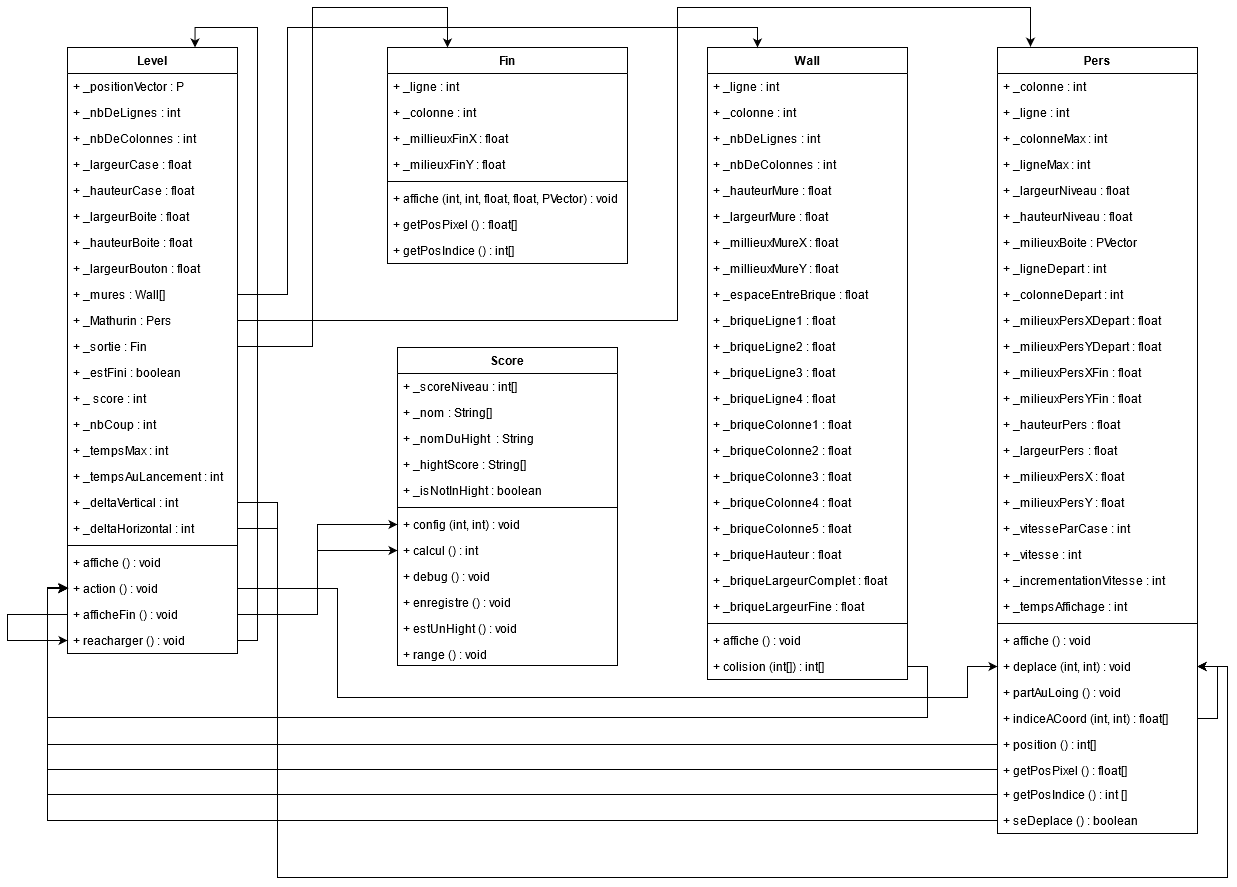
\includegraphics[width=1\textwidth]{Niveau.png}
  	\caption{Diagramme uml de la gestion d'un niveau}
  	\label{fig4}
\end{figure}
\subsection{Les popups}
Je me suis dit que des Popup seraient pratique pour avoir un retour de l'utilisateur. Pas compliqué dans l'ensemble étant donné que j'avais déjà des menu et une zone de saisie de texte que j'ai retiré par la suite pour la remplacé par des popups. Le plus gros problème étais de "bloquer" les interaction possible avec ce qui se trouvait derrière la popup. Dans un premier temps je voulais que la popup retourne du texte un peu comme \\
\verb| String toto = popup.feedback(numéos_de_popup);| \\
Mais je n'ai réussi à synchronisé tout ça j'ai donc fais en sort que ma popup modifie directement la valeur souhaité. 
\subsection{La class Text}
La manière dont j'ai géré mes fichiers texte était assez complexe. Et comme je ne voulais pas trop m'ennuyer à faire de code long, j'ai faire un objet texte qui n'est qu'un String[] mais sur lequel il y a pas mal d'action simple comme chercher une ligne ou retourner le caractère d'une lignes et d'un mot dans cette ligne. Je les aient utilisé à chaque fois que j'ai manipulé un fichier texte. 
\section{Conclusion}
Mon principal regrée est qu'il faille le rendre à une certaine date. sinon je l'aurais amélioré pendant des moins. J'ai notamment eu plein d'idées pour faire en sorte que l'éditeur soit le plus simple possible comme une vérification de la jouabilité, ou une génération procédurale de niveaux. De plus géré des niveau avec plusieurs personnage ou plusieurs sortie. Pour ce qui est du temps passé, je n'ai pas compté mais comme il s'agit de la 4 em refonte de tout le projet j'ai bien du y passer 80 h au moins. 

\end{document}